\section{Discussion}
\label{sec:discussion}

\subsection{Mass-dependent heating}

An alternative explanation for this phenomenon is that lower-mass stars
experience greater velocity changes when gravitationally perturbed and are
more efficiently dynamically heated.
Mass-dependent orbital heating has not been unambiguously observed in the
galactic disk because of the strong anti-correlation between stellar mass and
stellar age.
Less massive stars do indeed have larger velocity dispersions, however they
are also older on average.
This mass-age degeneracy is highly reduced in M dwarfs because their
main-sequence lifetimes are longer than the age of the Universe, however no
evidence for mass-dependent heating has been detected in these low mass stars
\citep{faherty2009}.

To investigate, we selected late K and M dwarfs observed by both \kepler\ and
\gaia, whose MS lifetimes exceed around 11 Gyrs and are therefore
representative of the initial mass function.
We could not perform this analysis on the sample of stars with measured
rotation periods, because only stars with {\it detectable} rotation periods
appear in the \mct\ catalog.
Since lower-mass stars stay active for longer it is likely that there are more
old stars (with larger velocity dispersions) at low masses in this sample.
% This allowed us to remove the degeneracy between mass and age that would
% confound evidence for mass-dependent heating among more massive stars.
% In a sample of massive stars with short MS lifetimes, lower-mass stars
% typically have greater velocity dispersion, but this could be either because
% dynamical heating is more efficient in lower mass stars, or because lower mass
% stars tend to be older because they live longer.
% In a sample of late K and M dwarfs, whose MS lifetime is longer than the age
% of the Universe, we can assume that none have evolved into giants and any
% additional heating seen in the lower-mass stars must be caused by
% mass-dependent heating.
We selected all \kepler\ targets with dereddened \gaia\ \gcolor\ colors
greater than 1.2 (corresponding to an effective temperature $\lesssim$
4800 K) and absolute \gaia\ $G$-band magnitudes $<$ 4.
We also eliminated visual binaries by removing stars above a 6th order
polynomial, fit to the MS on the \gaia\ CMD.
% shown in figure \ref{fig:mdwarf_CMD}.
We then applied the quality cuts described in section \ref{sec:the_data}.
% \begin{figure}
%   \caption{
% A \gaia\ color-magnitude diagram, showing all \kepler\ targets.
% We selected K and M dwarfs by applying color and magnitude cuts at \gcolor\ =
%     1.2 (\teff\ $\sim$ 4800 K) and $G$ = 4.
% We eliminated visual binaries by fitting a 6th order polynomial to the MS and
%     removing stars above it.
% Selected K and M dwarfs are shown as darker points.
% }
%   \centering
%     \includegraphics[width=1\textwidth]{mdwarf_CMD}
% \label{fig:mdwarf_CMD}
% \end{figure}
To search for evidence of mass-dependent heating we calculated the (\vb)
velocity dispersion of stars in effective temperature bins.
Again, sigma clipping was used to remove high velocity outliers before
calculating the standard deviation of stars in each bin.
% A slight excess of non-Gaussian outliers at lower temperatures leads to a
% marginal increase in velocity dispersion at low temperatures when sigma
% clipping is not performed.
% Figure \ref{fig:vb_vs_color} shows velocity and velocity dispersion as a
% function of \gaia\ \gcolor\ color.
% There is no clear trend between velocity dispersion and color.

Figure \ref{fig:vb_vs_teff} shows velocity and velocity dispersion
as a function of effective temperature (calculated by transforming dereddened
\gaia\ colors using equation \ref{eq:curtis}).
Velocity dispersion very slightly {\it decreases} with decreasing temperature,
(the opposite of the trend expected for mass-dependent heating) however the
slope is only inconsistent with zero at the 1.3 $\sigma$ level.
This trend may be due to a selection bias: cooler stars are fainter and
therefore typically closer, with smaller heights above the galactic plane and
smaller velocities.
The essential point here is that the increasing velocity dispersion with age
and decreasing temperature that is evident in figure \ref{fig:age_cut} is not
a result of an intrinsically larger velocity dispersion for low-mass stars.
We performed the same analysis on the 537 stars in this sample with RVs using
{\it vertical} velocity (\vz) and found the slope of the velocity
dispersion-temperature relation was consistent with zero.

Since we used \vb, not \vz\ in our analysis, it is possible that the
anti-correlation between \teff\ and galactic latitude, $b$, could influence
our results: stars at higher latitudes would have additional velocity
components in the ${\bf x}$ and ${\bf y}$ directions, which could increase
\vb\ but not \vz.
However, since the relationship between \sigmavb\ and \teff\ is positively,
not negatively correlated for cool stars in the \kepler\ field, this effect is
probably too small to influence our results.
% \begin{figure}
%   \caption{
%       Top: Stellar velocity (\vb) as a function of \gaia\ \gcolor\ color for
%       \kepler\ K and M dwarfs.
% Vertical lines indicate different color-groupings used to calculate velocity
%     dispersion.
% Pink stars were not included in velocity dispersion calculations as they were
%     removed as outliers during a sigma clipping process.
% Bottom: velocity dispersion as a function of color.
% There is no obvious trend between velocity dispersion and stellar color
%     indicating that mass-dependent heating does not significantly effect
%     low-mass stars in the \kepler\ field.
% }
%   \centering
%     \includegraphics[width=1\textwidth]{vb_vs_color}
% \label{fig:vb_vs_color}
% \end{figure}

\begin{figure}
  \caption{
      Top: Stellar velocity (\vb) as a function of \teff\ for
      \kepler\ K and M dwarfs.
Vertical lines indicate different \teff-groupings used to calculate velocity
    dispersion.
Pink stars were not included in velocity dispersion calculations as they were
    either removed as outliers during a sigma clipping process, or they lie at
    the sparcely populated, extremely cool end of the temperature range.
    Velocity dispersion and \teff\ are slightly positively correlated, likely
    due to a brightness-related selection bias, indicating that mass-dependent
    heating does not significantly affect low-mass stars in the \kepler\
    field.
}
  \centering
    \includegraphics[width=1\textwidth]{vb_vs_teff}
\label{fig:vb_vs_teff}
\end{figure}
Figure \ref{fig:vb_vs_teff} indicates that mass-dependent heating does not
strongly affect the \mct\ sample of rotating \kepler\ stars.
For this reason, we assume that age difference is the major cause of velocity
dispersion differences between groups.
In other words, (\vb) velocity dispersion is a reliable age proxy for the
\mct\ sample.

% The \vb\ AVR is not directly comparable to the \vz\ AVR, so, to draw a
% comparison with results from the literature, we calculated a \vz\ AVR for
% the subset of 290 cool stars in the \mct\ sample with \gaia\ RVs.
% We measured an AVR exponent of 0.47 $\pm$ 0.1, which falls within the range of
% values (0.45-0.53) reported from measurements of F and G stars in the Solar
% neighborhood \citep{holmberg2009, aumer2009, aumer2016}.
% It is a little lower than the values of 0.56 $\pm$ 0.14 (for low-z) and 0.51
% $\pm$ 0.15 (for high-z stars), calculated using \LAMOST\ \racomment{(LAMOST
% citation)} K giants \citep{yu2018}.
% K giants are more massive than K dwarfs \racomment{(how much more massive?)},
% so this slightly higher value contradicts the mass-dependent heating
% hypothesis.
% \racomment{Add some words about selection functions...}

% To investigate further, we calculated the exponent of the (\vb) AVR for each
% temperature bin in figure \ref{fig:age_cut}.
% \begin{figure}
%   \caption{
%       The exponent of the (\vb) AVR as a function of effective temperature.
% }
%   \centering
%     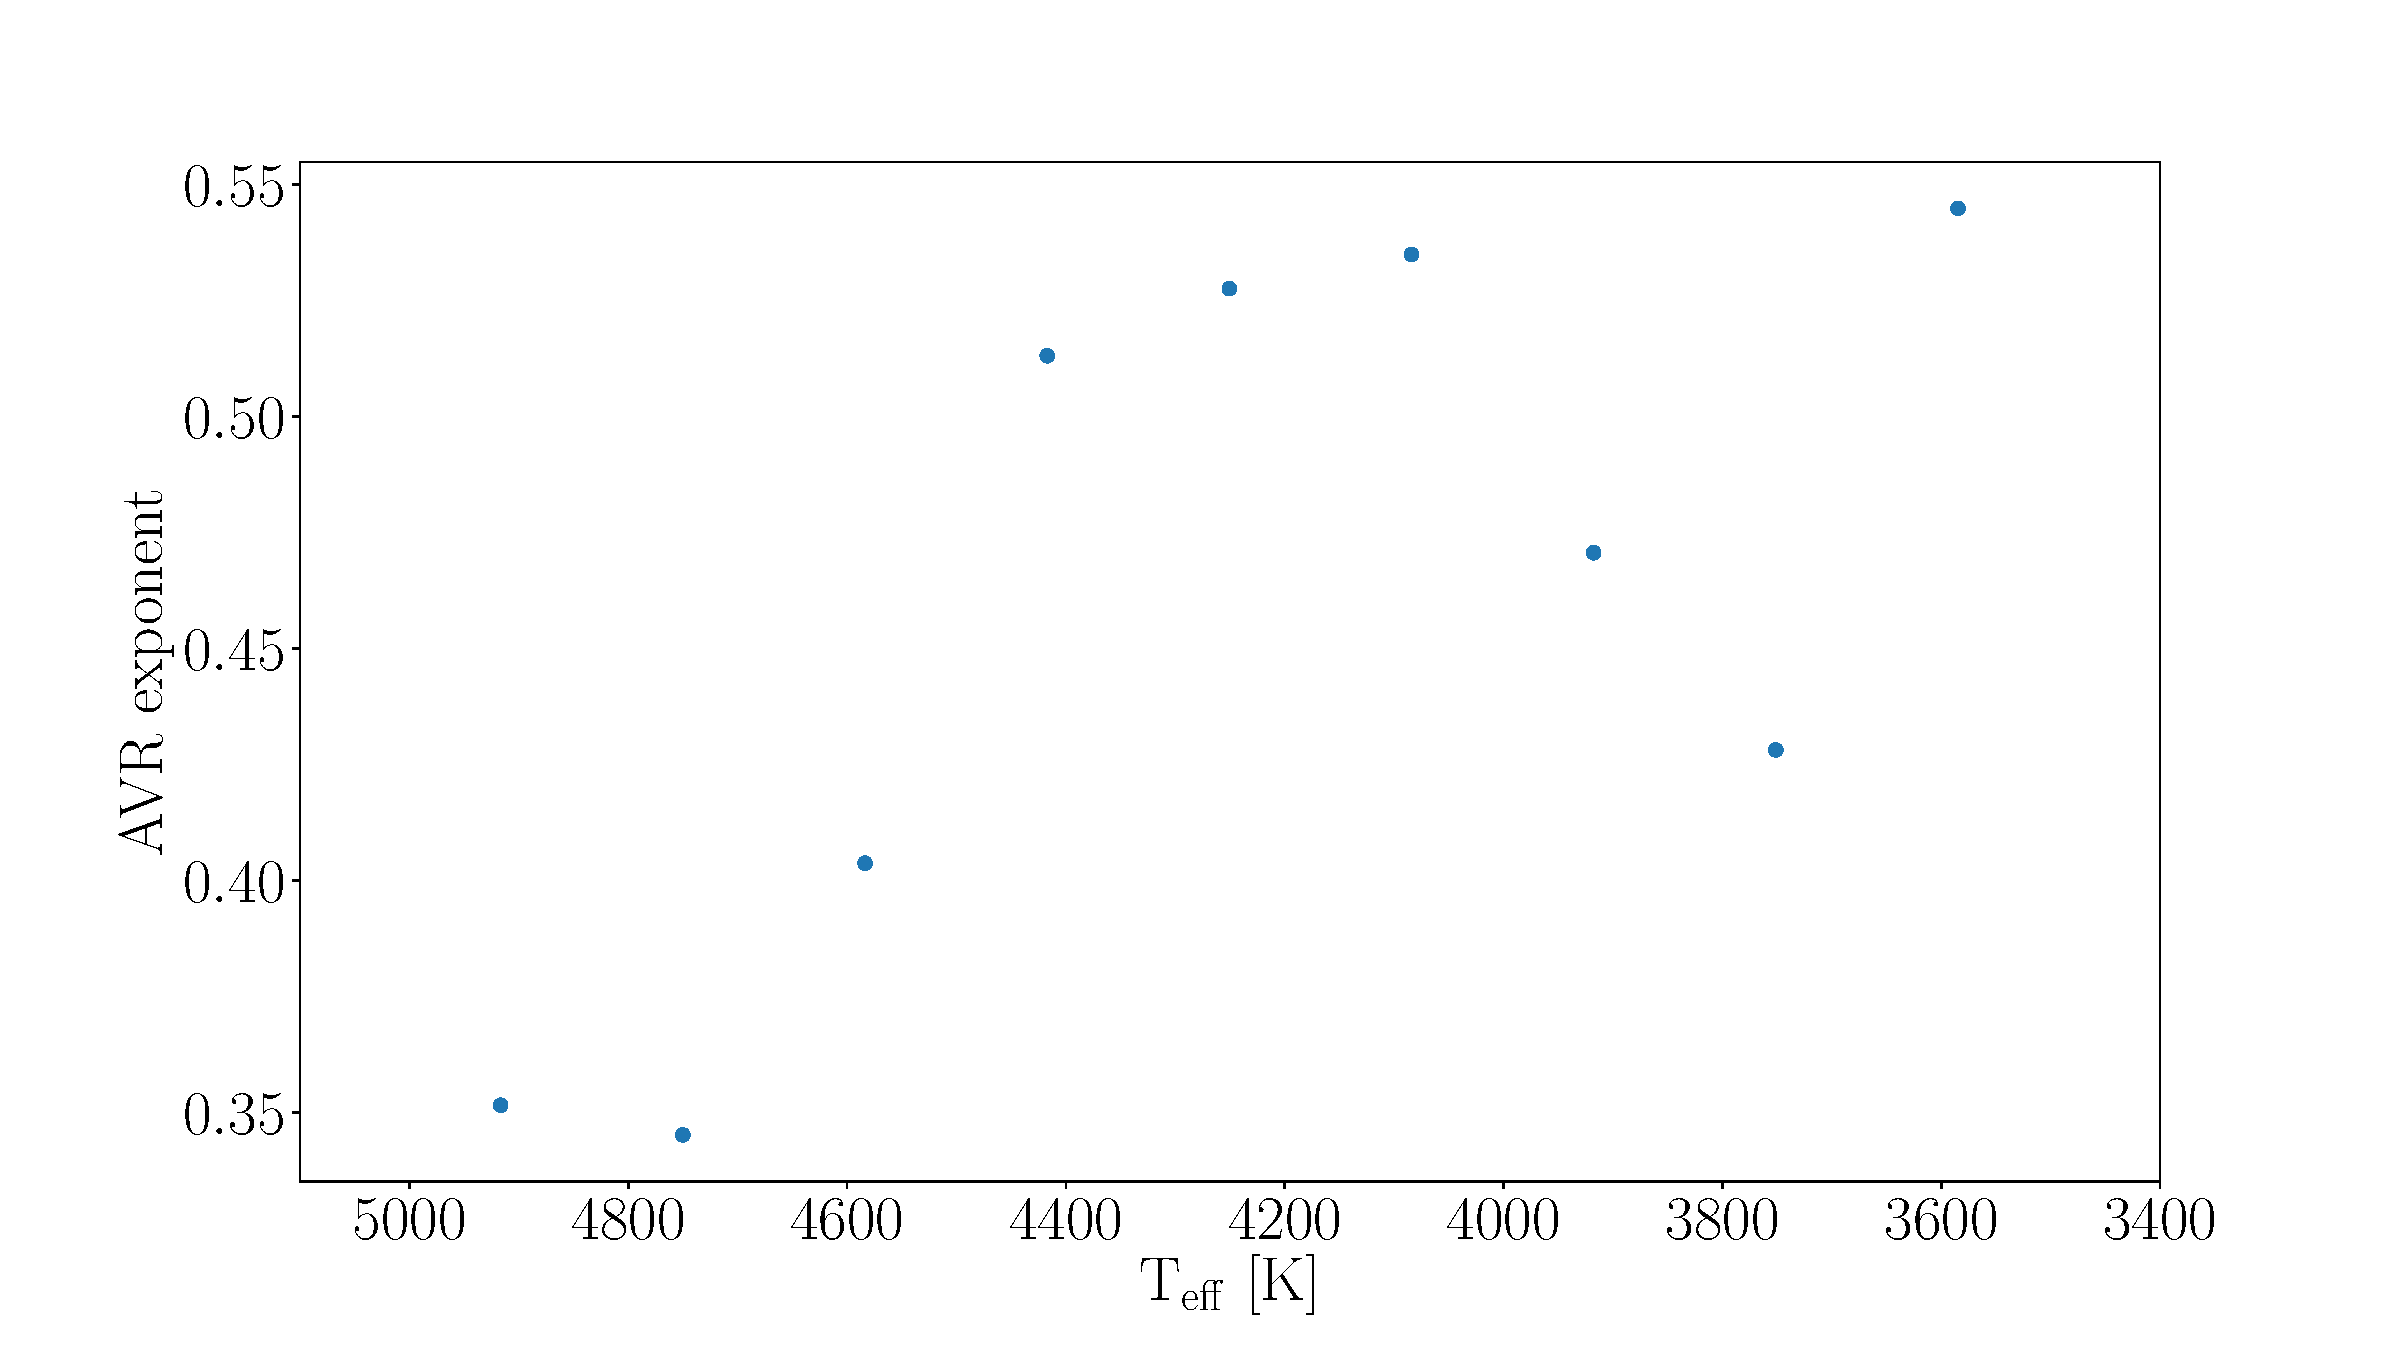
\includegraphics[width=1\textwidth]{AVR_exponent}
% \label{fig:AVR_exponent}
% \end{figure}
% Figure \ref{fig:AVR_exponent} shows the significant rise the in AVR exponent
% as a function of effective temperature.
% The hottest stars in our sample (\teff\ = 4833-5000 K) have a (\vb) AVR
% exponent of 0.39 $\pm$ 0.02 and the coolest (\teff\ = 3500-3667 K) have an
% exponent of 0.74 $\pm$ 0.02.
% The masses of stars in our sample differ by less than a factor of two,
% so mass-dependent heating cannot be entirely responsible for this large spread
% in heating rates.
% \racomment{Need to look into this further.}

% If mass-dependent heating is strongly affecting our data, the exponent of the
% AVR should increase with decreasing effective temperature, \ie\ the heating
% rate should be greater for lower-mass stars.
% Figure \ref{fig:AVR_exponent} shows the AVR exponent does indeed increase with
% decreasing effective temperature, however, the AVR exponent calculated using
% more massive stars from the Geneva Copenhagen Survey (GCS)
% \citep{holmberg2009} is also shown on this plot as a dashed horizontal line.
% Most GCS stars are F and G type: 1-3 times more massive than the K dwarfs used
% in our study.
% If mass-dependent orbital heating is the main cause the rise in velocity
% dispersion with decreasing \teff\ seen in figure \ref{fig:age_cut}, then the
% AVR exponent of the more massive GCS stars should fall {\it below} the AVR
% exponent for the most massive stars in our sample.
% In other words, the dynamical heating rate should be lowest for the highest
% mass stars and highest for the lowest mass stars.
% % nordstrom2004, jorgensen2005,
% These AVR exponents were calculated with different populations of stars,
% subject to different selection effects, so directly comparing them comes with
% some risk.
% The most important difference is that the GCS AVR is calculated using \vz,
% however our AVRs are calculated using \vb\ since most stars in our sample do
% not have radial velocities.
% The median galactic latitude of these \kepler\ stars is 12.3\degrees, with
% latitudes ranging from 5.5\degrees\ to 21.4\degrees, so \vb\ is a relatively
% close approximation to \vz.
% Only 290 out of the 6820 stars in our sample, plotted in color in figure
% \ref{fig:age_cut}, have \gaia\ radial velocities, however we used the ones
% that do to compare the \vz\ AVR to the \vb\ AVR, across all temperatures
% between 3500 and 5000 K.
% For stars with gyrochronal ages between 0.5 and 4.5 Gyr, we measured a \vz\
% AVR exponent of 0.519 $\pm$ ... and a \vb\ AVR exponent of 0.514 $\pm$... .
% The similarity of these two AVR exponents suggests that directly comparing
% these two quantities {\it may} be a reasonable approach.
% For now, given the large difference between the (\vz) AVR exponent of the GCS
% sample and the (\vb) AVR exponent of the hottest stars in our sample, we
% assume that the increased velocity dispersion at cooler temperatures is mostly
% caused by incorrect age-grouping due to an incorrect period-color relation at
% old ages, and that any mass-dependent heating, while it may contribute at a
% low level to this result, is not the dominant driver.
% However, differentiating the effects of mass-dependent heating and the shape
% of the gyrochronology relations is certainly warranted in a follow-up study.
% }

% Figure \ref{fig:age_comparison} shows the ages of star groups, predicted with
% the \citet{angus2019} gyrochronology relation, compared with the ages of star
% groups, predicted with the \citet{holmberg2009} AVR.
% \citet{holmberg2009} only provide an exponent (0.53), not an intercept, for the
% relation between logarithmic age (in Gyr) and logarithmic, \vz\ velocity
% dispersion (in \kms), so we fit the intercept to the mean \vb\ velocity
% dispersion across all temperatures, of our sample.
% \begin{figure}
%   \caption{
%       Ages predicted by the \citet{holmberg2009} \vz\ AVR, against ages
%     predicted by the \citet{angus2019} gyrochronology relation, for stars in
%     different temperature ranges.
% Points are colored by the effective temperature in the center of the \teff\
% bin.
% The dashed line shows the y=x relation.
% Predicted kinematic ages fan out over gyrochronal time, either because the AVR
%     is temperature-dependent or because the gyrochronology relations have an
%     age-dependent period-color relation.
% }
%   \centering
%     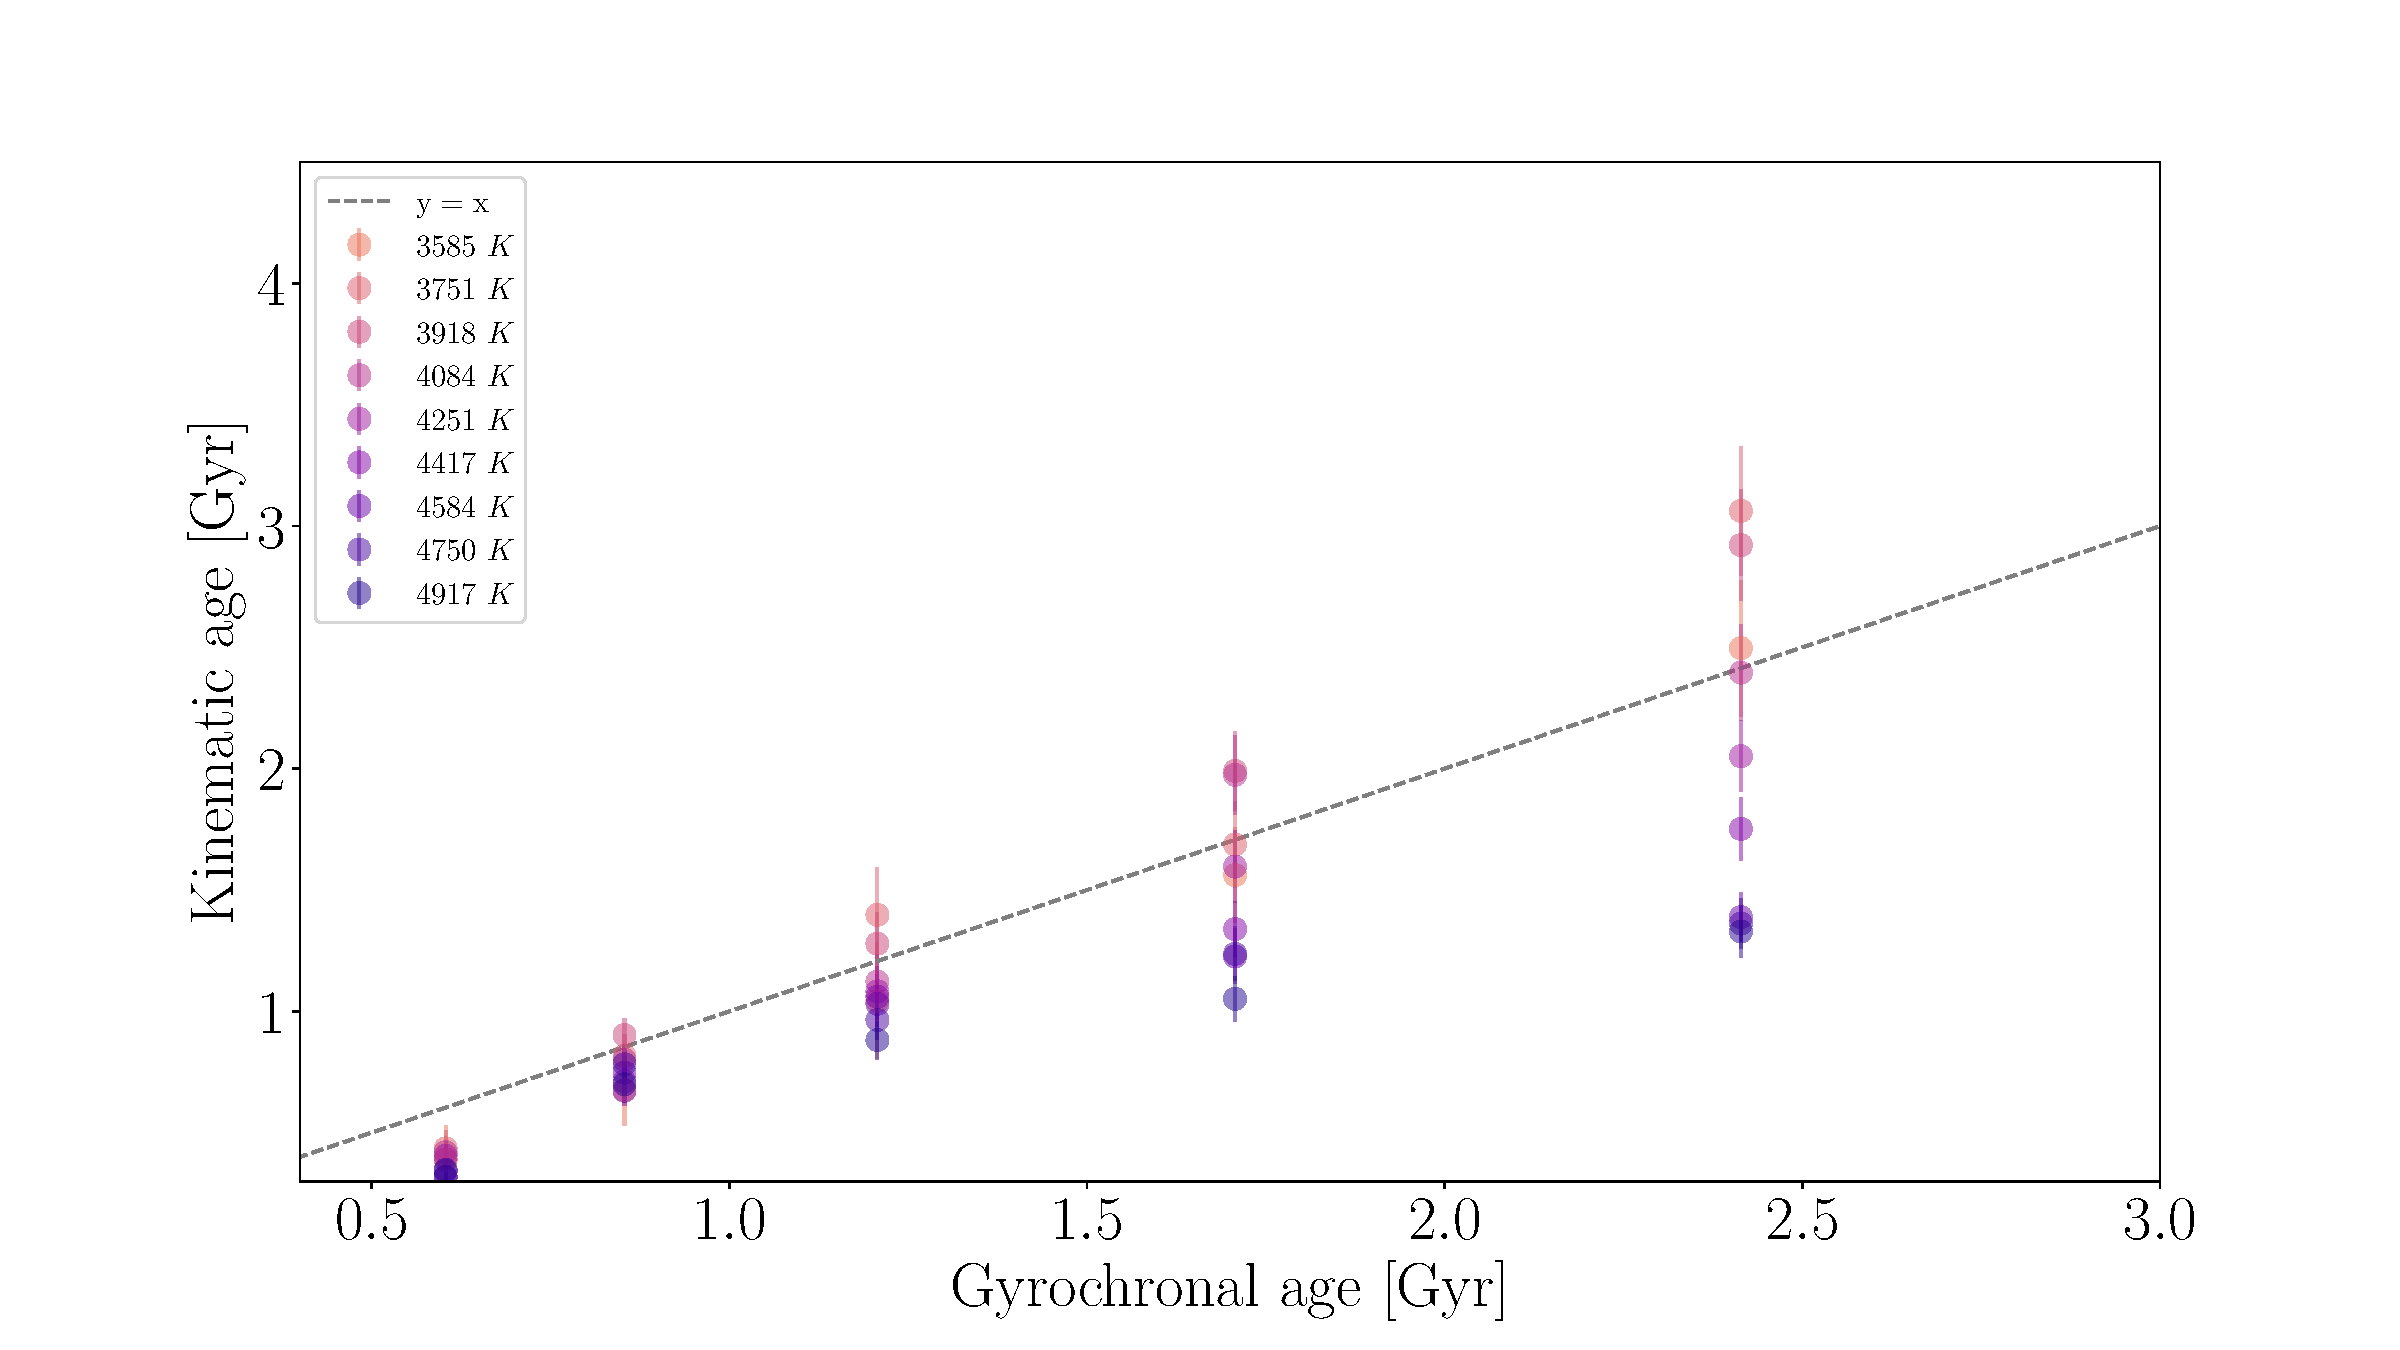
\includegraphics[width=1\textwidth]{age_comparison}
% \label{fig:age_comparison}
% \end{figure}
% Figure \ref{fig:age_comparison} shows a comparison between ages predicted by
% the \citet{holmberg2009} \vz\ AVR (using \vb\ as a proxy for \vz) and ages
% predicted by the \citet{angus2019} gyrochronology relation, for stars in
% different temperature ranges.
% The predicted kinematic ages fan out over gyrochronal time, either because the
% AVR is temperature-dependent or because the gyrochronology relations have an
% age-dependent period-color relation.
% Figure \ref{fig:age_comparion} also suggests that dynamical heating does not
% begin until after around ... Gyr:

% Alternatively, the ages of these young stars could be under-predicted by
% gyrochronology.
% These young stars have similar rotation periods to the Praesepe cluster, which
% was used to calibrate the gyrochronology relation used in this analysis.
% The ages of these young stars should, therefore, be the most accurate of the
% entire sample.
% However, they are tied to the age of the Praesepe cluster, whose age is not
% accurately known.
% \citet{angus2019} adopted an age for Praesepe of 650 Myrs, however the
% kinematic age-prediction for these stars is around 400 Myrs.
% Other studies have assigned a much older age of 800 Myrs to Praesepe
% \citep{brandt2015}.
% If the age assumed for Praesepe in the \citet{angus2019} gyrochronology
% calibration was inaccurate, the entire age {\it scale} would be incorrect.
% However, this is not what figure \ref{fig:age_comparion} shows -- it shows
% that the {\it relative} age of these youngest stars are under-predicted by
% kinematics or over-predicted by gyrochronology.

% If we assume that the rise in velocity dispersions at cooler effective
% temperatures is caused by an inaccurate period-color relation rather than
% mass-dependent dynamical heating, we can estimate what the shape of the
% period-color relations {\it should} be.
% Figure \ref{fig:age_cut} indicates that the period-color relation flattens
% out, so we applied the same analysis to groups of stars with similar rotation
% periods, equivalent to a completely flat period-color relation.
% The top panel of figure \ref{fig:period_cut} shows the \mct\ sample with stars
% in different period ranges plotted in different colors.
% The bottom panel shows the velocity dispersion of each group as a function of
% effective temperature.
% \begin{figure}
%   \caption{
% This figure is similar to figure \ref{fig:age_cut}, with stars divided into
%     period groups rather than age groups.
% The velocity dispersion is more constant across effective temperatures for the
%     most slowly rotating stars, compared to the stars selected with the
%     \citet{angus2019} gyrochronology model, indicating that the gyrochronology
%     models flatten out, and possibly even invert, at old ages.
% }
%   \centering
%     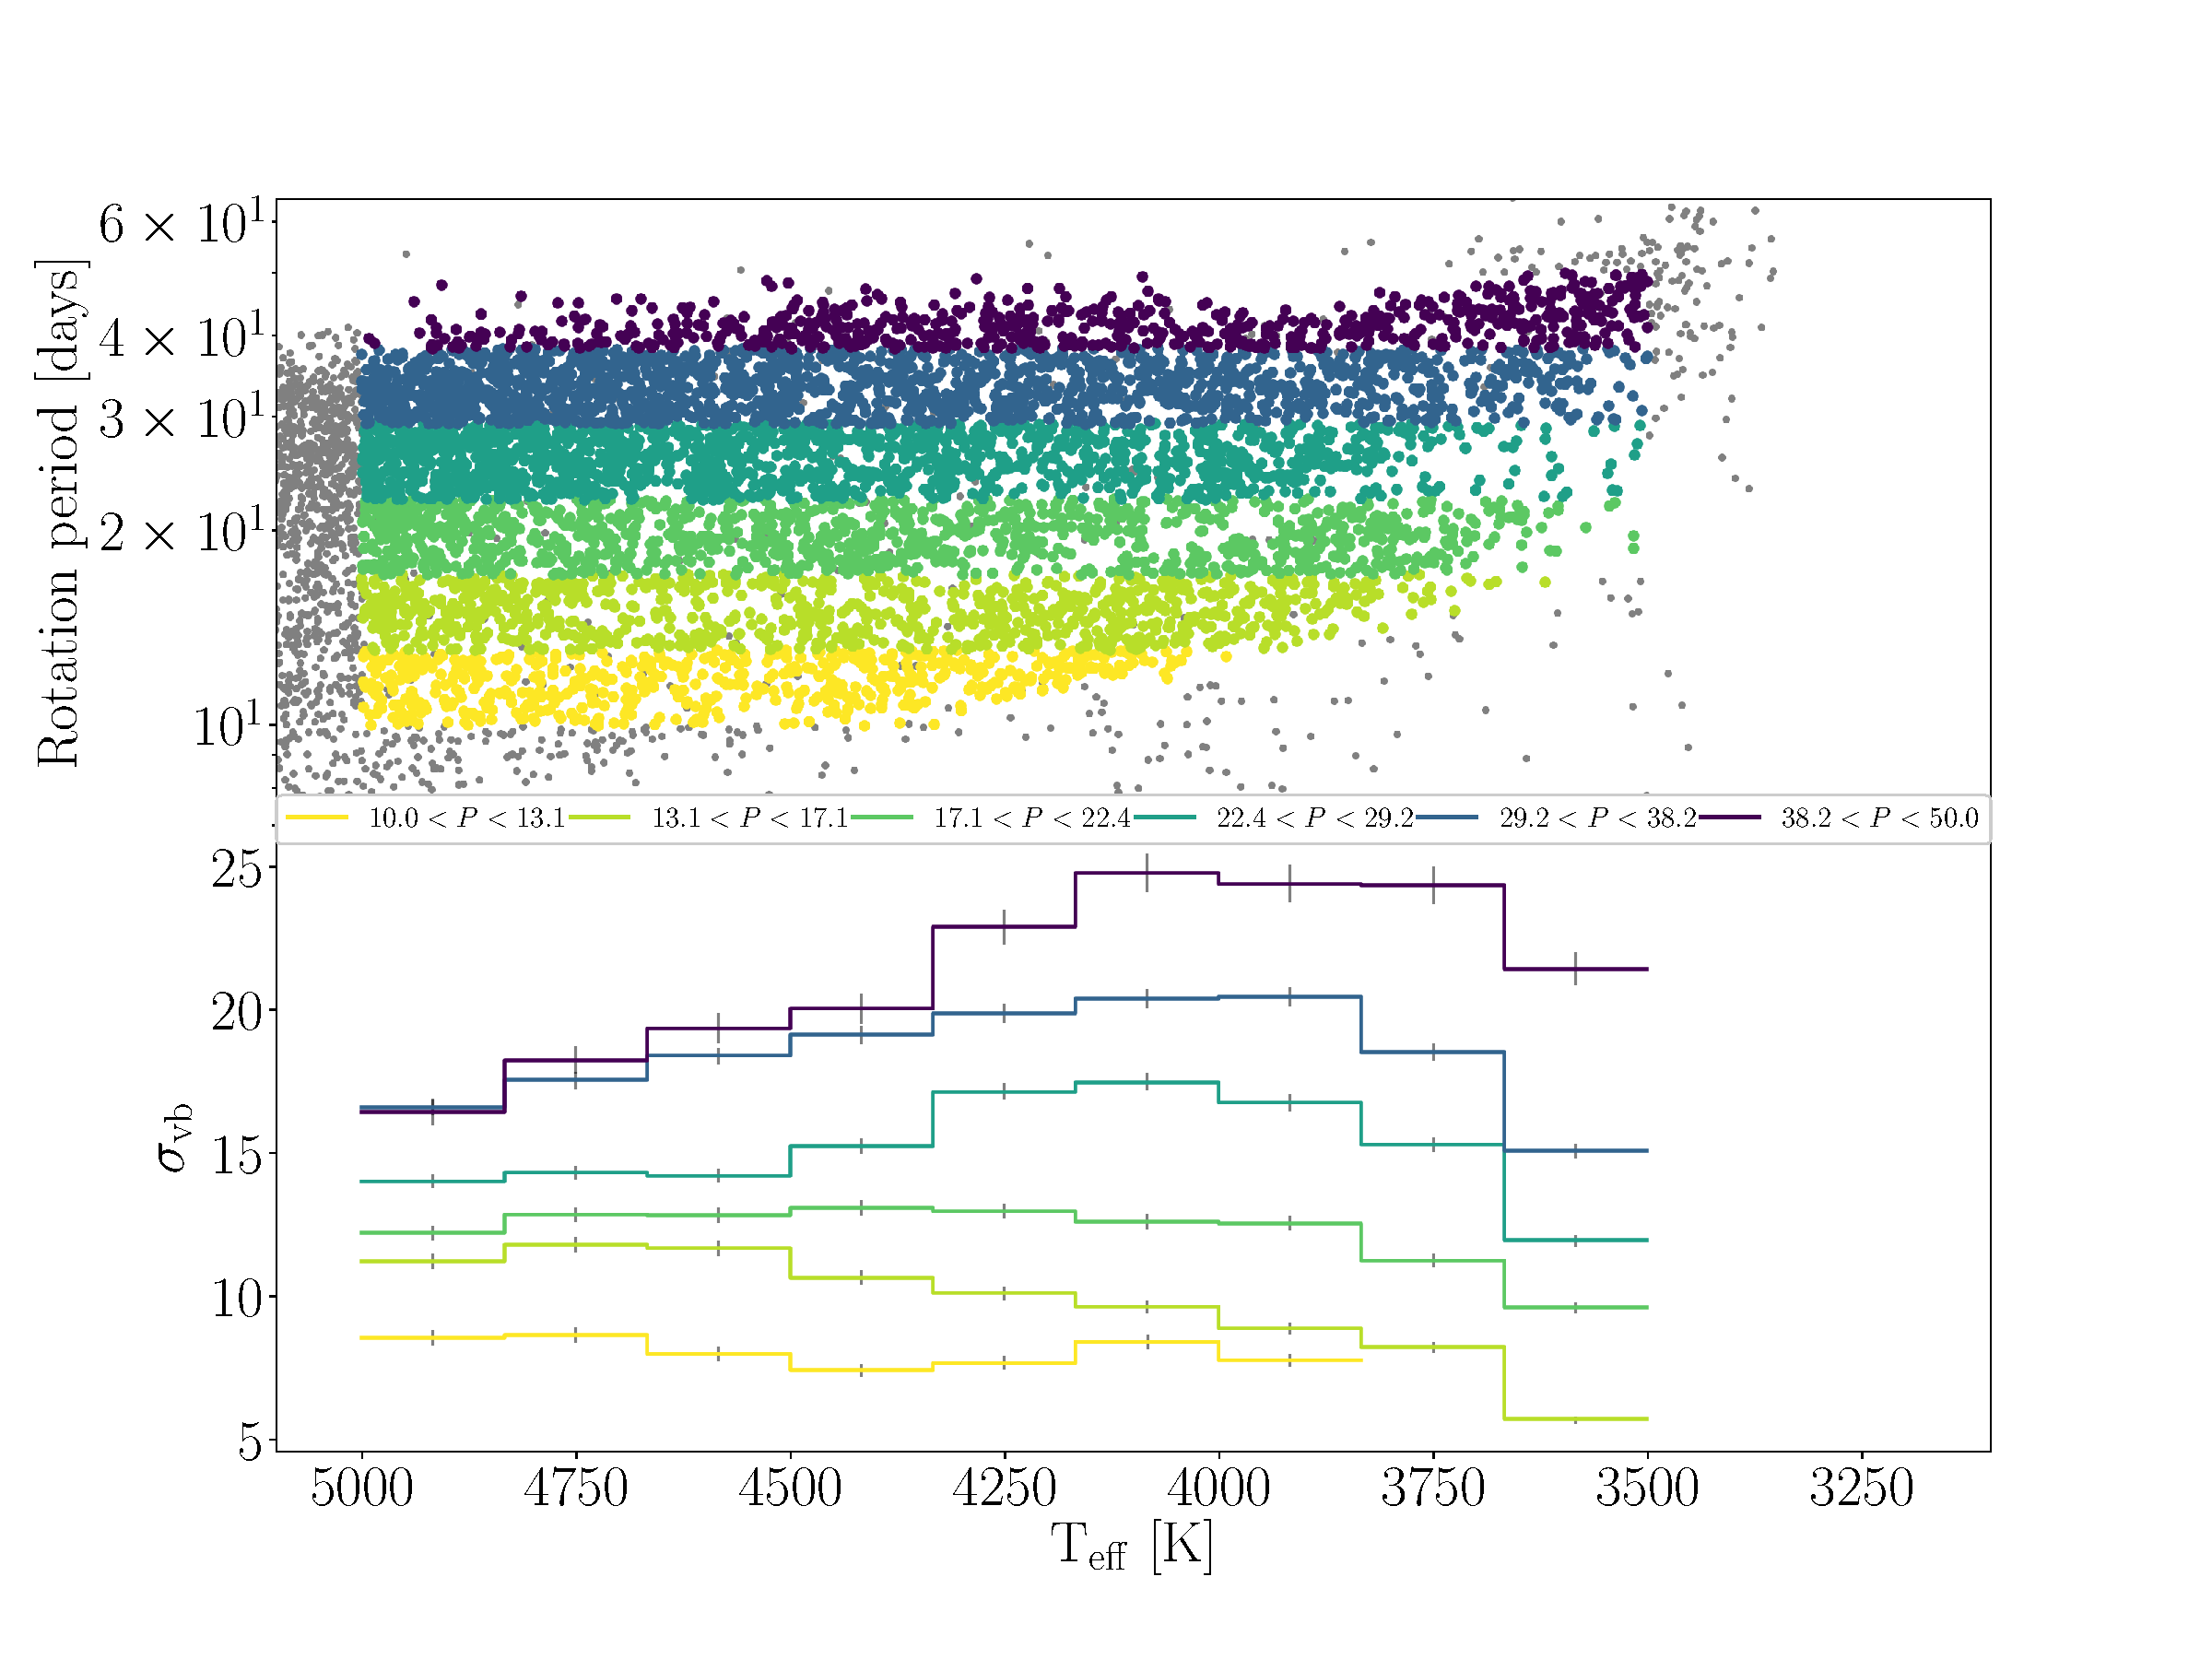
\includegraphics[width=1\textwidth]{period_cut}
% \label{fig:period_cut}
% \end{figure}
% Once again, the velocity dispersion increases with rotation period overall.
% For the most rapidly rotating groups of stars, velocity dispersion decreases
% with \teff\ as expected given the positively sloped period-color relation of
% Praesepe and other young clusters: late K dwarfs rotate more slowly than early
% K dwarfs of the same age.
% Between rotation periods of 15 and 25 days, the temperature dependence of the
% velocity dispersion starts to disappear, indicating that the period-color
% relation becomes flat: late K dwarfs rotate at the same rate as early K dwarfs
% of the same age.
% At long rotation periods, the velocity dispersion still increases with
% effective temperature, although the increase is much more modest compared to
% the oldest stars in figure \ref{fig:age_cut}.

% If we assume the rise in velocity dispersion at cooler effective temperatures
% is caused by an inaccurate period-color relation rather than mass-dependent
% dynamical heating, we can generate a graphical representation of what the
% relations {\it should} look like.

% Aside from the assumption that mass-dependent dynamical heating is {\it not}
% the main cause of the increased velocity dispersion for cooler stars, a number
% of assumptions went into this analysis which should be addressed before a
% strong conclusion about the nature of stellar spin down is drawn.
% There are some potential confounders that could produce trends between
% velocity dispersion and effective temperature, of which the main ones are
% listed below.
% \begin{itemize}

    % \item{{\bf Extinction.}
% Although we dereddened stars before their ages were estimated, if the
    %     reddening values were underestimated, the gyrochronal ages of stars
    %     would be under-estimated.
% This effect would be largest for the late Ks and early Ms, where the shape of
    %     the period-color relation is more steeply sloped, and stars can more
    %     easily move into the wrong age bin with a small perturbation in color
    %     or temperature.
% Old stars would be incorrectly assigned young ages, and this would happen more
    %     often for cooler stars.
% This effect could lead to an increase in velocity dispersion with \teff, even
% if the gyrochronology relation was perfect.}

    % \item{{\bf Mass-dependent orbital heating.}
% A key assumption going into this analysis is that the orbits of all stars are
% heated at the same rate, regardless of their mass.
% However, if the heating mechanism leads to preferential heating of lower mass
% stars, those stars would have a larger velocity dispersion, not caused by
% ageing.
% No strong evidence has yet been provided to show a mass-dependence in orbital
% heating, however this is an extremely difficult exercise because mass and age
% are so strongly correlated.
% The mass-age degeneracy is reduced in the lowest mass stars which represent
    %     the initial mass function of the Solar neighborhood.
% No mass-dependent heating was found by \citet{faherty2009} who looked
% at the velocity dispersions of low-mass stars.
% Another argument against the increased velocity dispersion as a function of
    %     \teff\ being caused by mass-dependent orbital heating, is that heating
    %     acts most strongly at young ages and most weakly at old ages, \ie\ on
    %     a logarithmic timescale.
% This is related to the fact that stars are more difficult to scatter once they
% are on orbits with a large out-of-plane component and they spend more time out
% of the mid-plane.
% Our data show the opposite trend: stars show little mass-dependent heating
    %     before around 1 Gyr.
% Moreover, the stars in the Geneva-Copenhagen study, used to calibrate the AVR
    %     \citep{holmberg2009} are F and G stars, around 1-3 times as massive as
    %     the K stars in our sample.
% % nordstrom2004, jorgensen2005,
% The ages for our sample of K stars, predicted by gyrochronology agree with the
    %     AVR calibrated using F and G stars, which implies that either
    %     mass-dependent heating is a weak effect, or, mass-dependent heating is
    %     strong and, by coincidence, gyrochronology underpredicts the ages of
    %     the early K dwarfs by just the right amount that they still appear to
    %     agree with the \citet{holmberg2009} AVR.
% We therefore expect that the increased velocity dispersion at cooler
    %     temperatures is mostly caused by incorrect age-grouping, \ie\ the
    %     period-color relation is incorrect for old, low-mass stars, and that
    %     any mass-dependent heating, while it may contribute at a low level to
    %     this result, is not the dominant cause.
% }

    % \item{{\bf Selection bias.}
% The \gaia\
% catalog is incompletebecause they are too faint.
% This is simply due to the fact that \kepler's field of view was aimed at low
    %     galactic latitudes, so nearby \kepler\ stars are close to the galactic
    %     plane.
% The heights of stars above the galactic plane, and correspondingly their
    %     velocities and ages, are therefore correlated with distance.
% Almost no high velocity stars appear in our sample at temperatures cooler than
% 3500, which is why the coolest stars were excluded from our sample, however
% the selection function could still affect stars hotter than 3500 K, and is
% suggested by the decrease in velocity dispersions for cool stars of all ages
% in figure \ref{fig:age_cut}.
% However, this selection effect would act in opposition to the observed trend.
% }

% \item{{\bf Weakened magnetic braking.}
% The rotation periods of old stars are faster than predicted by Skumanich-like
% magnetic braking \citep{angus2015, vansaders2016, metcalfe2019}.
% Magnetic braking is expected to become inefficient once stars approach a
% Rossby number (the ratio of rotation period to convective turnover time) of
% around 2 \citep{vansaders2016, vansaders2018}.
% Since hot stars have shallow convection zones and shorter overturn timescales,
% they reach $Ro = 2$ and stop spinning down at shorter rotation periods than
% cool stars.
% For this reason, some of the hotter stars in the sample may already have
% stopped spinning down, and could be much older than a traditional
% gyrochronology relation (like the simple Praesepe-based relation used in this
% analysis) would suggest.
% However, this effect would work to cancel out the trend observed in figure
% \ref{fig:age_cut} because hotter groups of stars would contain more old stars
% with large velocities.
% }

% \item{Stellar or exoplanet companions.}
% Hotter stars are more likely to be binaries.
% This would make synchronized some stars seem younger, more likely for massive
% stars, although really only likely at short rotation periods.

% \end{itemize}

\subsection{The period gap}
The origin of the rotation period gap, first identified
by \citet{mcquillan2013} and visible in figures \ref{fig:age_cut} and
\ref{fig:dispersion_period_teff} remains a mystery.
This gap can be seen as an under-density of points between the 0.7-1.0 and
1.0-1.5 Gyr age ranges in figure \ref{fig:age_cut} and roughly follows a line
of constant gyrochronal age of around 1.1 Gyr \citep[according to the
gyrochronology relation of][]{angus2019}, as shown in figure
\ref{fig:dispersion_period_teff}.
Several explanations for the gap's origin have been proposed, including a
discontinuous star formation history \citep{mcquillan2013, davenport2017,
davenport2018}, a rapid change in magnetic field structure
\citep{reinhold2019}, and erroneous rotation period measurements that are
incorrect by a factor of two \citep{koen2018}.
The latter explanation can be ruled out because stars below the gap have
smaller velocity dispersions than the stars above the gap, indicating that
they are kinematically younger \citep{mcquillan2013, davenport2018}, as
evident in figure \ref{fig:age_cut}.
For stars below the gap, in the 0.7-1.0 Gyr age range shown in figure
\ref{fig:age_cut}, velocity dispersion is relatively constant as a function of
temperature, however above the gap, in the 1.0-1.5 Gyr age range and older,
velocity dispersion increases with \teff.
The coolest stars in the 1.0-1.5 Gyr age range have the same velocity
dispersion as the hottest stars in the age range above which indicates that
the period-\teff\ relations are {\it flat} at these rotation periods.
This is also visible in figure \ref{fig:dispersion_period_teff}.
Below the gap, velocity dispersion within a given period range appears to {\it
decrease} with decreasing temperature.
The opposite appears to be true above the gap.

In the $\sim$ 1.1 Gyr NGC 6811 cluster, the rotation periods of mid-K dwarfs
are faster than expected; their rotational evolution appears to have stalled,
and the period-\teff\ relation is flat \citep{curtis2019}.
The rotation periods of the K dwarfs in this cluster are plotted in figure
\ref{fig:dispersion_period_teff}.
Although the G dwarfs in this cluster fall on the 1.1 Gyr gyrochronology
model, the K dwarfs lie only a little above the 0.65 Gyr gyrochronology model.
% If we assume that the gap is located at a single (gyrochronal) age, its age is
% remarkably similar to the NGC 6811 cluster (measured from MS turn-off) of 1.1
% Gyr \citep{meibom2011}.
NGC 6811 straddles the rotation period gap: its G dwarfs lie above it and its
K dwarfs lie below it.
This cluster may be the `missing link' that connects two epoch of stellar
spin-down: an early stage where the period-\teff\ relation for K dwarfs has a
negative slope and a late stage where it has a positive slope.
In this case the period gap may delineate the transition between these two
regimes and is the point at which stellar magnetic dynamos likely undergo a
dramatic structural shift at an age of $\sim$ 1.1 Gyr.

It may be a coincidence that the gyrochronology relations seem to only flatten
off {\it above} the period gap, or it may be that the period gap is located at
magnetic transition period.
We lack a sufficient quantity of data to investigate in detail but new field
star rotation periods from the \ktwo\ and \tess\ missions may be able to
validate or rule out this hypothesis in the future.
